%%%--- TITEL OG FORFATTER ---%%%
\newcommand{\tit}{Benchmarking the Lattice Boltzmann model implemented using NumPy and PyCUDA}
\newcommand{\aut}{Jens Bang \& Jacob Salomonsen}
\newcommand{\subj}{Bachelor Project}
\newcommand{\mail}{\href{mailto:jens@snej.dk}{jens@snej.dk} or \href{mailto:jiekebo@gmail.com}{jiekebo@gmail.com}}

%%%--- PREAMBLE INCLUDE ---%%%
%%%--- Preamble by Jacob Salomonsen ---%%%
\documentclass[a4paper,11pt]{article}

%%%--- IMPORT AF PAKKER ---%%%
\usepackage[hang,small,bf]{caption}		% Nice captions at figures
\usepackage[utf8]{inputenc}			% Input encoding
\usepackage[T1]{fontenc}				% Font encoding
\usepackage{amsmath}					% Matematiske kommandoer
\usepackage{amssymb}					% Matematiske symboler
\usepackage{amsfonts}					% Matematiske fonte
\usepackage{listings}					% Listing af kildekode
\usepackage{color}						% Color package used in listings
\usepackage{fancyhdr}					% Fancy header
\usepackage{booktabs}					% Flotte tabeller
\usepackage{color}						% Farver på listings
\usepackage{subfigure}					% Figurer i linje
%\usepackage{subfig}					% Figurer i linje
\usepackage{float}						% Customized floats
\usepackage{wrapfig}					% Tekst omkring figurer
\usepackage{tikz}							% Tikz tegning
\usetikzlibrary{automata,shadows,arrows,decorations.pathmorphing,backgrounds,positioning,fit}
\usepackage{pgf}							% Pgf tegning
\usepackage{hyperref}					% Hyper-links i PDF

%%%--- SKRIFTTYPE ---%%%
%\usepackage{stmaryrd}
%\usepackage{mathpazo}
%\usepackage{charter}
%\usepackage{helvet}
%\usepackage{avant}
%\usepackage{mathptmx}
%\usepackage{newcent}
%\usepackage{chancery}
%\usepackage{bookman}
%\usepackage{pifont}
%\usepackage{fourier}
%\usepackage{courier}

%%%--- HYPERREF SETUP ---%%%
\hypersetup{
    %bookmarks=true,					% show bookmarks bar?
    unicode=false,						% non-Latin characters in Acrobat�s bookmarks
    pdftoolbar=true,					% show Acrobat�s toolbar?
    pdfmenubar=true,					% show Acrobat�s menu?
    pdffitwindow=false,					% window fit to page when opened
    pdfstartview={FitH},				% fits the width of the page to the window
    pdftitle={\tit},					% title
    pdfauthor={\aut},					% author
    pdfsubject={Subject},				% subject of the document
    pdfcreator={Creator},				% creator of the document
    pdfproducer={Producer},				% producer of the document
    pdfkeywords={keywords},				% list of keywords
    pdfnewwindow=true,					% links in new window
    colorlinks=true,					% false: boxed links; true: colored links
    linkcolor=blue,						% color of internal links
    citecolor=blue,						% color of links to bibliography
    filecolor=blue,						% color of file links
    urlcolor=blue						% color of external links
}

%%%--- 1,5 LINJEAFSTAND ---%%%
%\linespread{1,3}

%%%--- SIDE LAYOUT ---%%%
\addtolength{\textwidth}{2.0cm}
\addtolength{\evensidemargin}{1.0cm}
\addtolength{\oddsidemargin}{-1.0cm}
\setlength{\parindent}{0.0cm}
\setlength{\headheight}{16pt}
%\textheight = 20.5cm
%\hoffset
%\voffset
%\oddsidemargin = 18pt
%\topmargin = 0pt
%\headheight = 13.6pt
%\headsep = 25pt
%\textheight = 646pt
%\textwidth = 424pt
%\marginparsep = 11pt
%\marginparwidth = 54pt
%\footskip = 30pt
%\marginparpush = 5pt
%\hoffset = 0pt
%\voffset = 0pt
%\paperwidth = 597pt
%\paperheight = 845pt

%%%--- STANDARD TITLEPAGE ---%%% (Husk \maketitle)
\title{\tit}
\author{\aut}
\date{\today}

%%%--- MACRO INPUT ---%%%
%%%%%%%%%%%%%%%%%%%%%%%%%%%%%%%%%%%%%%%%%%%%%%%%%%%%%%%%
%%              Jacob Salomonsens Macros              %%
%%%%%%%%%%%%%%%%%%%%%%%%%%%%%%%%%%%%%%%%%%%%%%%%%%%%%%%%
%%%%%%%%%%%%%%%%%%%%%%%%%%%%%%%%%%%%%%%%%%%%%%%%%%%%%%%%
%%                       Layout                       %%
%%%%%%%%%%%%%%%%%%%%%%%%%%%%%%%%%%%%%%%%%%%%%%%%%%%%%%%%

\newcommand{\HRule}		{\rule{\linewidth}{0.5mm}}

\newcommand{\insfig}[4]{		% \insfig{path}{scale}{caption}{label}
\begin{figure}[H]
	\begin{center}
		\includegraphics[width=#2]{#1}
		\caption{#3}
		\label{#4}
	\end{center}	
\end{figure}
}

\newcommand{\instbl}[3]{		% \instbl{tabular}{caption}{label}
\begin{table}[htb]
	\begin{center}
		#1
		\caption{#2}
		\label{#3}
	\end{center}
\end{table}
}

%%%%%%%%%%%%%%%%%%%%%%%%%%%%%%%%%%%%%%%%%%%%%%%%%%%%%%%%
%%                        Math                        %%
%%%%%%%%%%%%%%%%%%%%%%%%%%%%%%%%%%%%%%%%%%%%%%%%%%%%%%%%

\newcommand{\maple}[2]{			% Til formatering af maple input, 1=kommando 2=output
\\\\\indent\texttt{[>#1}		% Brug \\ i output til at lave flere linier.
\begin{center}
\texttt{#2}
\end{center}
}

\newcommand{\matr}[4]{			% \matr{[}{]}{colums}{contents (\\ = change row)}
\left#1\!\begin{array}{#3}
#4
\end{array}\!\right#2
}

\newcommand{\Rm}[1]		{\mathrm{#1}}
\newcommand{\unit}[1]		{\ensuremath{\,\mathrm{#1}}}
\newcommand{\NN}		{\ensuremath{\mathbb N}}
\newcommand{\RR}		{\ensuremath{\mathbb R}}
\newcommand{\CC}		{\ensuremath{\mathbb C}}
\newcommand{\degree}		{\ensuremath{\,^{\circ}}}
\newcommand{\tii}[1]		{\ensuremath{\cdot10^{#1}}}
\newcommand{\vekt}[1]		{\ensuremath{\overrightarrow{#1}}}
\newcommand{\result}[1]		{\underline{\underline{#1}}}
\newcommand{\rd}		{\mathrm{d}}
\newcommand{\E}			{\mathrm{e}}
\newcommand{\I}			{\mathrm{i}}

%%%%%%%%%%%%%%%%%%%%%%%%%%%%%%%%%%%%%%%%%%%%%%%%%%%%%%%%
%%                      Physics                       %%
%%%%%%%%%%%%%%%%%%%%%%%%%%%%%%%%%%%%%%%%%%%%%%%%%%%%%%%%

\newcommand{\std}[1]		{#1^{\minuso}}
\newcommand{\stdm}[1]		{#1^{\minuso}_\Rm{m}}
\newcommand{\dstd}[2]		{\Delta_\mathrm{#1} #2^{\minuso}}

\newcommand{\dQ}		{\rd Q}
\newcommand{\dS}		{\rd S}
\newcommand{\dT}		{\rd T}
\newcommand{\dH}		{\rd H}
\newcommand{\dU}		{\rd U}
\newcommand{\dV}		{\rd V}
\newcommand{\dP}		{\rd p}
\newcommand{\dG}		{\rd G}
\newcommand{\dTau}		{\rd \tau}
\newcommand{\dN}		{\rd N}
\newcommand{\dn}		{\rd n}

\renewcommand{\DH}		{\Delta H}
\newcommand{\DG}		{\Delta G}
\newcommand{\DU}		{\Delta U}
\newcommand{\DS}		{\Delta S}
\newcommand{\DV}		{\Delta V}
\newcommand{\DT}		{\Delta T}
\newcommand{\DM}		{\Delta \mu}


\newcommand{\pstd}		{p^{\minuso}}
\newcommand{\sstd}		{S^{\minuso}}
\newcommand{\smstd}		{S_\Rm{m}^{\minuso}}

\newcommand{\cpstd}		{C_p^{\minuso}}
\newcommand{\cpmstd}		{C_{p,\Rm{m}}^{\minuso}}
\newcommand{\cpm}		{C_{p,\Rm{m}}}
\newcommand{\cp}		{C_{p}}

\newcommand{\cvstd}		{C_V^{\minuso}}
\newcommand{\cvmstd}		{C_{V,\Rm{m}}^{\minuso}}
\newcommand{\cvm}		{C_{V,\Rm{m}}}
\newcommand{\cv}		{C_{V}}

\newcommand{\Hm}		{H_\Rm{m}}
\newcommand{\kb}		{k_\Rm{B}}
\newcommand{\jpk}		{\unit{J}\unit{K^{-1}}}
\newcommand{\jm}		{\unit{J}\unit{mol^{-1}}}
\newcommand{\jkm}		{\unit{J}\unit{K^{-1}}\unit{mol^{-1}}}
\newcommand{\kj}		{\unit{kJ}}
\newcommand{\kjm}		{\unit{kJ}\unit{mol^{-1}}}
\newcommand{\gpm}		{\unit{g}\unit{mol^{-1}}}

\newcommand{\Tfus}		{T_\Rm{fus}}
\newcommand{\Tvap}		{T_\Rm{vap}}
\newcommand{\Tm}		{T_\Rm{m}}
\newcommand{\Tb}		{T_\Rm{b}}
\newcommand{\TRoom}		{298.15 \unit{K}}
\newcommand{\TMelt}		{273.15 \unit{K}}
\newcommand{\Kstd}		{\std{K}}

\newcommand{\Q}[2]		{#1 \unit{#2}}

%%%%%%%%%%%%%%%%%%%%%%%%%%%%%%%%%%%%%%%%%%%%%%%%%%%%%%%%
%%                     Chemistry                      %%
%%%%%%%%%%%%%%%%%%%%%%%%%%%%%%%%%%%%%%%%%%%%%%%%%%%%%%%%

% \reak{\chem{HCl}&+&\chem{NaOH}&$\rightarrow$&\chem{NaCl}&+&\chem{H_2O}}
\newcommand{\reak}[1]{
\begin{center}
	\begin{tabular}{ccccccccccccccccc}
		#1
	\end{tabular}
\end{center}
}

\newcommand{\chem}[1]	{\ensuremath{\mathrm{#1}}}
\newcommand{\lra}		{\longrightarrow}
\newcommand{\arr}		{\rightleftarrows}
\newcommand{\darr}		{\rightleftarrows}
\newcommand{\KS}		{\textrm{K}_s}
\newcommand{\KB}		{\textrm{K}_b}
\newcommand{\KV}		{\textrm{K}_v}
\newcommand{\mol}		{\textrm{mol}}
\newcommand{\g}			{\textrm{g}}
\newcommand{\gm}		{\frac{\g}{\mol}}
\newcommand{\M}			{\textrm{M}}
\newcommand{\konc}		{\frac{\mol}{\textrm{L}}}
\newcommand{\pH}		{\textrm{pH}}
\newcommand{\pOH}		{\textrm{pOH}}

%%%%%%%%%%%%%%%%%%%%%%%%%%%%%%%%%%%%%%%%%%%%%%%%%%%%%%%%%%%%%%%%%%%%%%%%
%% Chemical species
%%%%%%%%%%%%%%%%%%%%%%%%%%%%%%%%%%%%%%%%%%%%%%%%%%%%%%%%%%%%%%%%%%%%%%%%
\newcommand{\ammnitrats}{\chem{NH_4NO_3(s)}}
\newcommand{\benzen}    {\chem{C_6H_6}}
\newcommand{\borto}     {\chem{B_2}}
\newcommand{\bor}       {\chem{B}}
\newcommand{\brmal}     {\chem{BrCH(COOH)_2}}
\newcommand{\brma}      {\chem{BrMA}}
\newcommand{\brmsf}     {\chem{{\sf [BrMA]}}}
\newcommand{\bromat}    {\chem{BrO_3^-}}
\newcommand{\bromid}    {\chem{Br^-}}
\newcommand{\brom}      {\chem{Br^-}}
\newcommand{\brsyr}     {\chem{HBrO_2}}
\newcommand{\brto}      {\chem{Br_2}}
\newcommand{\calc}      {\chem{Ca^{2+}}}
\newcommand{\cefsf}     {\chem{{\sf [Ce^{4+}]}}}
\newcommand{\cef}       {\chem{Ce^{4+}}}
\newcommand{\cet}       {\chem{Ce^{3+}}}
\newcommand{\chloridc}  {\chem{[Cl^-]}}
\newcommand{\clto}      {\chem{Cl_2}}
\newcommand{\cltog}     {\chem{Cl_2(g)}}
\newcommand{\carbon}    {\chem{C}}
\newcommand{\carbongr}  {\chem{C(grafit)}}
\newcommand{\chlorid}   {\chem{Cl^-}}
\newcommand{\coto}      {\chem{CO_2}}
\newcommand{\cotos}     {\chem{CO_2(s)}}
\newcommand{\cotol}     {\chem{CO_2(l)}}
\newcommand{\cotog}     {\chem{CO_2(g)}}
\newcommand{\co}        {\chem{CO}}
\newcommand{\fe}        {\chem{Fe}}

\newcommand{\hbro}      {\chem{HBrO}}
\newcommand{\hoclc}     {\chem{[HOCl]}}
\newcommand{\hocl}      {\chem{HOCl}}
\newcommand{\hoic}      {\chem{[HOI]}}
\newcommand{\hoi}       {\chem{HOI}}
\newcommand{\hpc}       {\chem{[H^+]}}
\newcommand{\hp}        {\chem{H^+}}

\newcommand{\htooc}     {\chem{[H_20]}}
\newcommand{\htoo}      {\chem{H_2O}}
\newcommand{\htoog}     {\chem{H_2O(g)}}
\newcommand{\htool}     {\chem{H_2O(l)}}
\newcommand{\htoos}     {\chem{H_2O(s)}}
\newcommand{\hcl}       {\chem{HCl}}
\newcommand{\hclg}      {\chem{HCl(g)}}

\newcommand{\hto}       {\chem{H_2}}
\newcommand{\htog}      {\chem{H_2(g)}}
\newcommand{\htol}      {\chem{H_2(l)}}
\newcommand{\htos}      {\chem{H_2(s)}}

\newcommand{\iodidc}    {\chem{[I^-]}}
\newcommand{\iodid}     {\chem{I^-}}
\newcommand{\ipt}       {\chem{IP_3}}
\newcommand{\mal}       {\chem{CH_2(COOH)_2}}
\newcommand{\ma}        {\chem{MA}}
\newcommand{\ethan}     {\chem{C_2H_6}}
\newcommand{\ethang}    {\chem{C_2H_6(g)}}
\newcommand{\methan}    {\chem{CH_4}}
\newcommand{\methang}   {\chem{CH_4(g)}}
\newcommand{\mn}        {\chem{Mn}}
\newcommand{\naphtalen} {\chem{C_{10}H_8}}
\newcommand{\nhtre}     {\chem{NH_3}}
\newcommand{\nhtreg}    {\chem{NH_3(g)}}
\newcommand{\ntoog}     {\chem{N_2O(g)}}
\newcommand{\nto}       {\chem{N_2}}
\newcommand{\ntog}      {\chem{N_2}}
\newcommand{\oclmc}     {\chem{[OCl^-]}}
\newcommand{\oclm}      {\chem{OCl^-}}
\newcommand{\ohmc}      {\chem{[OH^-]}}
\newcommand{\ohm}       {\chem{OH^-}}
\newcommand{\oimc}      {\chem{[OI^-]}}
\newcommand{\oim}       {\chem{OI^-}}

\newcommand{\oto}       {\chem{O_2}}
\newcommand{\otog}      {\chem{O_2(g)}}
\newcommand{\ozon}      {\chem{O_3}}
\newcommand{\ozong}     {\chem{O_3(g)}}

\newcommand{\phenol}    {\chem{C_6H_5OH}}
\newcommand{\rut}       {\chem{Ru}}
\newcommand{\sotog}     {\chem{SO_2(g)}}
\newcommand{\sotol}     {\chem{SO_2(l)}}
\newcommand{\sotos}     {\chem{SO_2(s)}}
\newcommand{\soto}      {\chem{SO_2}}

\newcommand{\sns}       {\chem{Sn(s)}}
\newcommand{\snotos}    {\chem{SnO_2(s)}}

%%%%%%%%%%%%%%%%%%%%%%%%%%%%%%%%%%%%%%%%%%%%%%%%%%%%%%%%%%%%%%%%%%%%%%%%
%% References
%%%%%%%%%%%%%%%%%%%%%%%%%%%%%%%%%%%%%%%%%%%%%%%%%%%%%%%%%%%%%%%%%%%%%%%%

\newcommand{\hpref}[2]{\hyperref[#2]{#1 \ref{#2}}}

%%%%%%%%%%%%%%%%%%%%%%%%%%%%%%%%%%%%%%%%%%%%%%%%%%%%%%%%%%%%%%%%%%%%%%%%
%% Custom environments
%%%%%%%%%%%%%%%%%%%%%%%%%%%%%%%%%%%%%%%%%%%%%%%%%%%%%%%%%%%%%%%%%%%%%%%%

\newfloat{grammar}{thp}{lop}
\floatname{grammar}{Grammar}

%\usepackage[danish]{babel}				% Dansk orddeling osv.
%\usepackage[fixlanguage]{babelbib}		% Sprogpakke til BibTeX
%\selectbiblanguage{danish}				% Sprogvalg til BibTeX

%%%--- LISTISTINGS SETUP ---%%%
\lstset{ %
language=C++, 							% choose the language of the code
basicstyle=\footnotesize,				% the size of the fonts that are used for the code
numbers=left,							% where to put the line-numbers
numberstyle=\footnotesize,				% the size of the fonts that are used for the line-numbers
stepnumber=2,							% the step between two line-numbers. If it's 1 each line will be numbered
numbersep=5pt,							% how far the line-numbers are from the code
backgroundcolor=\color{white},			% choose the background color. You must add \usepackage{color}
showspaces=false,						% show spaces adding particular underscores
showstringspaces=false,					% underline spaces within strings
showtabs=false,							% show tabs within strings adding particular underscores
frame=single,							% adds a frame around the code
tabsize=2,								% sets default tabsize to 2 spaces
captionpos=b,							% sets the caption-position to bottom
breaklines=true,						% sets automatic line breaking
breakatwhitespace=false,				% sets if automatic breaks should only happen at whitespace
escapeinside={\%*}{*)}					% if you want to add a comment within your code
}

%%%--- FANCYHDR ---%%%
\pagestyle{fancy}
\chead{}
\lhead{\aut}
\rhead{\nouppercase{\leftmark}}
\cfoot{}
\lfoot{\today}
\rfoot{\thepage}

%%%--- DOKUMENT STARTER HER ---%%%
\begin{document}

%%%--- Title ---%%%%
\begin{titlepage}
\HRule
\begin{center}\huge{\bfseries{\tit}}\end{center}
\HRule
\\[1.0cm]
\begin{center}
\aut
\\[0.5cm]
\mail
\\[0.5cm]
\subj
\\[1.5cm]
Department of Computer Science
\\[0.5cm]
University of Copenhagen
\end{center}
\vfill
\begin{center}\today\end{center}
\end{titlepage}

%%%--- Tekst ---%%%

\section{Abstract}
To implement blablalba

\section{Introduction}
The intention of this project blablalba....

Reference tests:

Cuda by example\cite{cudabyexample}

\newpage
\tableofcontents
\newpage

\section{Theory}

\subsection{Lattice Boltzmann Model (\textit{Jens Bang})}
The Lattice Boltzmann Model (LBM) is a simplified version of the Boltzmann equation, which simulates the behaviour of fluid flows. The simplification consists of limiting the particles to only occupy certain points in space (vertices in a lattice), and to only travel along specified directional vectors, with constant speed. 

In this way the Lattice Boltzmann Model (LBM) describe simple fluids (gas and liquids), i.e. it ignores thermal effects and tracers. The LBM simulates movements in fluids by looking at particles found at points in a lattice at discrete time-steps. There are different versions of the LBM using either 2-dimensional or 3-dimensional lattices.

Each point in the lattice has a set of state-variables attached, describing the state of the particle found at that point. Each point also has a set of fixed directions, along which the particle can travel. In a 2-dimensional lattice there are normally 9 directions, while in a 3-dimensional lattice you see either 15 or 19 directions. These 3 setups are normally referred to as D2Q9, D3Q15 and D3Q19.

\insfig{./images/d2q9_d3q19.png}{0.5\textwidth}{LBM directions (TODO: Insert reference to Scholarpedia)}{lbmdirections}

The LBM divides the flow of gasses or fluids into small, discrete time-steps. For each time-step the algorithm traverses all lattice points and for each point calculates the velocity and direction the particle travels in, as well as handling any collisions between particles.

\subsubsection{Using the LBM}
Since the LBM is especially well suited to simulate flows around even very complex geometric structures, it has a wide variety of practical uses. Among these are:
\begin{itemize}
\item Simulating pore-scale processes in porous media [@@@@Ref: BrittSBChristensenPhD-Thesis.pdf]
\item Windmills [@@@@Mangler ref]
\item Andet?
\end{itemize}

\subsection{CPU vs. GPU}
  Different goals produce different designs !   GPU assumes work load is highly parallel !   CPU must be good at everything, parallel or not
!   CPU: minimize latency experienced by 1 thread !   big on-chip caches !   sophisticated control logic
!   GPU: maximize throughput of all threads
!  
!   !  
threads in flight limited by resources => lots of resources (registers, bandwidth, etc.)
multithreading can hide latency => skip the big caches share control logic across many threads

\subsection{Parallel processing}

\subsection{CUDA (\textit{Jacob Salomonsen})}
In the beginning, GPU's had only very limited purposes. Mostly generating real-time graphics for games, but also in a few cases for production and scientific applications. This has changed since the proliferation of the pixel shader. A pixel shader basically produces a color for every point on a screen, taking (x,y) position of the pixel, light settings of a scene, material properties and so on. Early researchers found that this ability to perform computations on each pixel could be harnessed to other uses. Since pixel shaders are completely controlled by the programmer the possibility of simply giving a GPU data as input, instead of a scene to render, was within reach. This would mark the beginning of the general purpose GPU.

The general purpose GPU did however lack a platform for developers to build upon, since learning to program pixel shaders required previous knowledge about either openGL or DirectX. Also even when knowing these frameworks, the model would lack the perspective of general purpose computing and instead be focused on generating graphics, where the general purpose computing aspect would be achieved by "cheating" the GPU into treating data as if it was a scene to be rasterized.

Enter CUDA. CUDA is nVidia's way of introducing general purpose GPU programming to a wider audience. CUDA utilizes the parallel nature of the GPU, allowing a low end computer to process data in a different and some times more efficient way.

The CUDA API exposes a set of tags which allows a programmer to easily specify what methods, in otherwise ordinary c-code, should be executed on the GPU. The way CUDA makes it possible is by using a preprocessor which parses the source code and makes different files for the individual architectures. Thus the normal c-code goes to whichever compiler the user chooses, and the parallel section of the code goes to a compiler specifically designed to generate PTX-code. PTX-code is essentially assembly which is not specific to any GPU. The PTX code is then translated into assembly code specifically targeted at the GPU.

This effectively separates the tedium of writing assembly code directly aimed at a specific GPU-architecture, or writing pixel shaders via graphics APIs.

\subsubsection{CUDA programming model}
The CUDA programming model efficiently supports the steps needed to be taken in order to make a process parallel. The model is arranged so a decomposition of the problem area is naturally ingrained in the programming procedure, by having the programmer split the problem into parts. Since the GPU is capable of launching many threads it is necessary to have control of what thread is launching where. Therefore nVidia has structured execution of code in a way that both allows an easy intuition of the GPU-architecture as well as supporting the steps in making a process parallel.

The code to be executed on the GPU, called the kernel henceforth, launches a grid which contains blocks of threads. A kernel can only launch one grid at a time. Blocks can be two-dimensionally arranged and the threads within the blocks can be arranged three-dimensionally. Threads within blocks can cooperate via shared memory, but cannot cooperate with threads from another block. It is therefore pivotal for the performance of a parallel process that a domain analysis has been made and the memory intensive parts of the problem are contained within a block.

Blocks do not only have the role of sharing memory among treads. It also serves as a synchronization point for the threads within it. A special command within CUDA will issue that all threads within a block must have completed before further execution is permitted.

To support this structure, CUDA provides built-in facilities for indexing blocks and threads. This allows the programmer to write code specifically for a single thread within a grid of many blocks, together containing millions of threads.

(TODO: make figure to show how grid and block structure can be in cuda)

\insfig{./images/cudaprocess.png}{0.5\textwidth}{CUDA process model (from Wikipedia article, author: Tosaka)}{cudaprocess}

\subsubsection{CUDA data model}

\insfig{./images/cudamem.png}{0.5\textwidth}{CUDA(GPU) memory model (TODO: where did I get this from?!)}{cudamem}

\newpage

\section{Implementation (\textit{Jacob Salomonsen})}


\subsection{Matlab implementation analysis}\label{sec:matlabimplementation}
The NumPy (\hpref{listing}{lbmnumpy}) and CUDA (\hpref{listing}{lbmcuda}) implementations take origin in a Matlab script (\hpref{listing}{lbmmatlab}). The analysis has been made on the D2Q9 version, but the D3Q19 is just an extension of this with an extra dimension. Since the project relies on a black-box implementation scheme, it was necessary to first perform an analysis of the supplied script. The first step taken in the analysis was to map what each of the key variables purpose were. The result can be seen in \hpref{table}{matlabvars}

\begin{table}[htb]
	\centering
	\begin{tabular}{llp{6cm}}
		\toprule
		Variable & Type & Purpose \\
		\midrule
		\texttt{F} 				& $nx\times ny\times 9$ (double)	& eight directional matrices and one stationary state matrix\\
		\texttt{FEQ} 			& $nx\times ny\times 9$ (double)	& equilibrium state of the nine matrices\\

		\texttt{BOUND} 			& $nx\times ny$ (binary) 		& boundary defined by 1's ($b$)\\
		\texttt{CI}				& $8\times 1$ (integer) 			& linear index of directional matrices\\
		\texttt{ON}				& $b\times 1$ (integer)			& linear index of obstacle nodes\\
		\texttt{TO\_REFLECT}		& $b\times 8$ (integer)			& linear index of nodes to save to BOUNCEBACK over all nine matrices\\
		\texttt{REFLECTED} 		& $b\times 8$ (integer) 			& linear index of nodes to recover from BOUNCEBACK over all nine matrices \\
		\texttt{BOUNCEBACK}		& $b\times 8$ (integer) 			& densities bouncing back\\
		\texttt{DENSITY}			& $nx\times ny$ (double) 		& summation of all nine matrices\\
		\texttt{UX}				& $nx\times ny$ (double) 		& summation of all densities with non zero x-component\\
		\texttt{UY}				& $nx\times ny$ (double) 		& summation of all densities with non zero y-component \\
		\texttt{U\_SQU}			& $nx\times ny$ (double) 		& sum of UX squared and UY squared\\
		\texttt{U\_C2}			& $nx\times ny$ (double) 		& sum of UX and UY\\
		\texttt{U\_C4}			& $nx\times ny$ (double) 		& negative sum of UX and UY\\
		\texttt{U\_C6}			& $nx\times ny$ (double) 		& negative of U\_C2\\
		\texttt{U\_C8}			& $nx\times ny$ (double) 		& negative of U\_C4\\
		\bottomrule
	\end{tabular}
	\caption{Variables and their purpose in the Matlab version of D2Q9 LBM}
	\label{matlabvars}
\end{table}

The main and most important variable in the script is the \texttt{F}-variable. From \hpref{table}{matlabvars} we see that \texttt{F} is a $nx\times ny\times 9$ matrix. This means that it has the size of the simulated field, and nine states of the the simulated fields. Hence according to the theory section this variable stores eight density directions and one stationary state. 

The secondary result of the variable analysis was a clearer understanding of the procedures taking place upon running the Matlab script. The script can be divided into four separate parts: \textbf{Propagation}, \textbf{Density}, \textbf{Equilibrium}, \textbf{Bounce-back}.

\subparagraph{Propagation} 
Propagation is where node densities are spread outward to affect neighbouring nodes. In the Matlab code this happens in line 44-55 in \hpref{listing}{lbmmatlab}. Lets examine line 45 and see how this is done

\begin{verbatim}
>> F(:,:,1)=F([nx 1:nx-1],:,1);
\end{verbatim}

On the right hand side a new matrix is created from \texttt{F}, by simply re-indexing the original array. Basically if the simulated field is $nx=10$ wide the statement \texttt{[nx 1:nx-1]} creates the following

\begin{verbatim}
10     1     2     3     4     5     6     7     8     9
\end{verbatim}

Essentially propagating the data in an eastward direction, by wrapping the end of the matrix around and shifting the rest forward, corresponding to vector c1 in \hpref{figure}{lbmdirections}. The rest of the expression says to go along all elements of the second axis, and only operate on matrix one out of nine. One thing to keep in mind when analysing Matlab code is that it uses one-based indexing, as opposed to most programming languages (e.g. Python) which uses zero-based indexing.

The rest of the propagation part of the script is simply an extension of the above, with the only difference being the direction of the propagation, by shifting the indices appropriate to the matrix in question.

\subparagraph*{Density}
The first task done in the density part (line 57-61 in \hpref{listing}{lbmmatlab}) of the Matlab script is the saving of densities bouncing back from obstacles. The way this is done is a little involved so it deserves some attention.

On line 21 of \hpref{listing}{lbmmatlab} the variable \texttt{CI} is generated, and as stated in \hpref{table}{matlabvars} the variable is the linear index of the first element of the 1--8 matrices (matrix 9 is not used for bounce-back). This means that if the simulated field is $10\times10$ the indices would be

\begin{verbatim}
0   100   200   300   400   500   600   700
\end{verbatim}

Combined with the variable \texttt{ON}, which contains the linear index for obstacle nodes, this can be used to calculate the linear position of obstacle nodes, in all of the 1--8 matrices.

The indices of obstacles in matrix 1--8 is saved in the variable \texttt{TO\_REFLECT} and then used to access all positions within the \texttt{F}-variable where there exists an obstacle, bearing in mind that this is the same position per obstacle for each 1--8 matrix, only with different linear indices.

The density is easily calculated by use of the sum command, which sums the matrices up along the third axis, i.e. the density matrices 1--9 are reduced to one.

The \texttt{UX} and \texttt{UY} variables are created by summing only the entries in the density matrices, where the x- or y-component respectively are non-zero. The meaning of x- and y-component is illustrated in \hpref{figure}{uxuy}.

\insfig{./images/uxuy.pdf}{0.7\textwidth}{The \texttt{UX} and \texttt{UY} variables are created}{uxuy}

\subparagraph*{Equilibrium}
The equilibrium part that runs from 63--88 of \hpref{listing}{lbmmatlab} increases the inlet pressure as to create a constant flow in the simulation. This part also uses the result from the density part to calculate some constants used in calculation of the equilibrium. The equilibrium is calculated for each density matrix 1--9, the first one being the stationary state as seen below.

\begin{verbatim}
FEQ(:,:,9)=t1*DENSITY.*(1-U_SQU/(2*c_squ));
\end{verbatim}

Here the special '.' operator is used, signifying that it is an element-by-element operation, not an operation on the full matrix.

Subsequently the \texttt{FEQ}-variable is added to the \texttt{F}-variable

\subparagraph*{Bounce-back}
The final part bounce-back is done just like at our first encounter with bounce-back, in the density part where it is saved, only this time the directions have been shifted. The operation is on line 91 of \hpref{listing}{lbmmatlab} The \texttt{REFLECTED} variable is just like \texttt{TO\_REFLECT}, with the difference for example being that density matrix 1 has been swapped with density matrix 5, which is in the opposite westward direction compared to the original direction. Taking this example, looking at \hpref{figure}{uxuy}, F1 is the original direction and the inverse direction is F5. This pattern of inverting is applied for all density matrices, effectively sending density in the opposite direction of the obstacle.



\subsection{NumPy}
NumPy is a scientific computing package for Python, which allows for multidimensional arrays, and routines for fast operations on these arrays. NumPy was used in implementing the CPU-version of the D2Q9-LBM. NumPy has the disadvantage that it will only run on one CPU, even in a multi-core processor (TODO: add reference for this). This severely limits the potential for scientific computing using this package, but the usefulness of this package is that it is easy to prototype calculations.

At the core of the NumPy package is the \textit{ndarray}. The \textit{ndarray} is a statically allocated data structure, which after creation cannot change in size. If an attempt to change the size of an existing array is made, the existing array is simply overwritten. To allocate an array fitting the data layout (discussed in part in \autoref{sec:matlabimplementation} and \autoref{sec:datalayout}), the following command is used:

\begin{verbatim}
>>> F = numpy.zeros((9,nx,ny), dtype=float)
\end{verbatim}

This allocates a three dimensional array consisting of zeros. Here the first dimension spans 9 indices, and the other two dimensions span the given width and height of the simulated field. The \texttt{dtype} parameter decides what data-type is to be used, in this case a float of no specification. 

As an alternative an array can be allocated with ones instead of zeros, which is useful for generating the scenery in the simulation field. This is simply done by the command

\begin{verbatim}
>>> BOUNDi = numpy.ones(BOUND.shape, dtype=float)
\end{verbatim}

Arrays have certain attributes attached to them, which can be accessed by the dot operator. In the command above it can be seen that one of these attributes, .shape, is accessed to create a new array with the same shape as another array. Here the meaning of the command is to create an array consisting of ones called \texttt{BOUNDi} in the shape of \texttt{BOUND}, i.e. with the same dimensions as \texttt{BOUND}.

When dealing with data in an euclidean space it is important to remember that the array class in NumPy is column major. Therefore methods for example used for plotting data will expect the first dimension of a two-dimensional array to correspond with the y-axis of a normal plot. 

NumPy supports summation operations so as to be able to reduce the nine directional matrices. This is done by the use of the command

\begin{verbatim}
>>> DENSITY = numpy.add.reduce(F)
\end{verbatim}

Which produces the result of adding all the matrices along the first dimension, i.e. the nine separate directional matrices. This could of course have been done even if the first dimension was not the directional matrices but instead the x-axis of the simulated field. Then an argument would have to be given to the \texttt{add.reduce} command to tell it along which axis to sum.

\begin{verbatim}
>>> DENSITY = numpy.add.reduce(F, axis=2)
\end{verbatim}

To expand a matrix by a new dimension, which is needed for the boundary calculations. Since the boundary matrix is only two dimensional it is necessary to expand upon it to be able to impose the boundary on the directional matrices. This is done by the command

\begin{verbatim}
>>> BOUND[numpy.newaxis,:,:]
\end{verbatim}



\subsection{PyCUDA}
PyCUDA is an extension for the Python language, that allows for full access to the functionality available to CUDA C. Since Python is a scripting language, which means it is not compiled but interpreted, the programming process is leveraged. The work-flow of PyCUDA is shown in \hpref{figure}{pcwork}. One notable advantage over CUDA C is automatic resource control. Another advantage is the tight coupling with NumPy, which is especially good for the main purpose of this paper. The testing procedure will also gain more reliability by keeping the execution on the same platform.

\insfig{./images/pycudaworkflow.pdf}{1.0\textwidth}{PyCUDA work-flow (from \cite{kloeckner_pycuda_2009})}{pcwork}

PyCUDA allows a programmer trained in the usage of CUDA C, to easily start programming. Basically PyCUDA allows for CUDA C-code to be embedded into the Python script. This is afforded by the \texttt{SourceModule}, which is a command used for creating CUDA kernels. A kernel is defined as a string like this

\begin{verbatim}
mod = SourceModule("""
__global__ void multiply_them(float *dest, float *a, float *b)
{
  const int i = threadIdx.x;
  dest[i] = a[i] * b[i];
}
""")
\end{verbatim}

This is just ordinary CUDA C, embedded in the Python code. To get the handle for the kernel this is done

\begin{verbatim}
multiply_them = mod.get_function("multiply_them")
\end{verbatim}

Now \texttt{multiply\_them} can be called like any normal Python function and the kernel will run with the arguments supplied in the call. When passing parameters as constant, it is easy to string replace them into the kernel before it gets turned into a CUDA kernel. An example of this is shown in \hpref{listing}{minikernel}

\lstset{language=Python, caption={An example of a kernel implemented in PyCUDA, here showing how constants are supplied on compile time},label=minikernel}
\begin{lstlisting}
constant = 10

mult_string = """
__global__ void multiply_them(float *dest, float *a, float *b) {
    const int i = threadIdx.x;
    dest[i] = a[i] * b[i] * %(CONSTANT)s;
}
"""

mult_string = mult_string % {
    'CONSTANT': constant
}

mod = SourceModule(mult_string)
\end{lstlisting}

Here the \texttt{\%(CONSTANT)s} is the label for the location for replacement of the string with the defined constant \texttt{constant} containing the value 10. This is done right after the kernel string by assigning a value to the label \texttt{'CONSTANT'}. As usual the string is sent as argument to the \texttt{SourceModule} and the kernel is ready to go.

As with CUDA C it is also necessary to load data onto the GPU by first allocating space and then copying to the GPU-memory. PyCUDA allows for allocating memory on the GPU using the \texttt{driver.mem\_alloc} command, with argument for the size of the memory to allocate. This command will allocate global memory on the GPU, which is the memory both the CPU and GPU can read and write to (TODO: check whether the copy is just for a pointer to the python buffer or if data is loaded into gpu-memory). Copying to the GPU is performed with the \texttt{device.memcpy\_htod}. Copying back from the GPU is afforded by the command \texttt{driver.memcpy\_dtoh}.

When creating variables in NumPy, meant to be transferred to the GPU by PyCUDA, it is important to specify a data-type the GPU will accept. For example to specify what kind of float type a new array should be created with, the command from the NumPy section can be augmented with the following statement

\begin{verbatim}
>>> F = numpy.zeros((9,nx,ny), dtype=float).astype(numpy.float32)
\end{verbatim}

The \texttt{astype} ensures data is allocated as 32-bit floats, which are especially suited for CUDA.

PyCUDA allows for allocation to different memory types on the GPU as seen in \hpref{figure}{cudamem}. We have already covered global memory. What remains is one of the CPU read/write GPU read memories, Texture-memory. Texture-memory is a special kind of memory which exhibits a spatial characteristic. This means that data most suited for this memory is either two or three dimensional. This memory is relatively fast compared with the global memory, but the drawback is that seen from the GPU it is read only. The allocation and usage is reminiscent of the CUDA C method. As with CUDA C a texture is defined in the kernel, which is contained within PyCUDA's \texttt{SourceModule}

\begin{verbatim}
texture<float, 2> tex;
\end{verbatim}

Now as with CUDA C the texture reference is tied to the texture's 'name' in the kernel

\begin{verbatim}
texture_func = mod.get_function("kernel_handle")
texref = mod.get_texref("tex")
\end{verbatim}

Now the that the reference has been set up, it is possible to load data into the texture. Loading a matrix into the texture is done like this

\begin{verbatim}
>>> pycuda.driver.matrix_to_texref(a, texref, order="C")
\end{verbatim}

Here the \texttt{a} is used for the kernel call, and exists on the GPU-side. The last parameter decides what order the dimensions are, if it is 'C' then \texttt{tex2D(x,y)} is going to fetch \texttt{matrix(y,x)}, otherwise if 'F' \texttt{tex2D(x,y)} is going to fetch \texttt{matrix(x,y)} (TODO: cite the pycuda manual).

A very clever feature in PyCUDA is the GPUArray class. The GPUArray behaves like the \textit{ndarray}, but performs it's computations on the GPU instead of one CPU-core. To create an empty GPUArray, a, using an \textit{ndarray}, x, as a template the following command can be used

\begin{verbatim}
a = gpuarray.empty_like(x)
\end{verbatim}

To copy an existing \textit{ndarray} to the GPU using the GPUArray class, the following command can be used.

\begin{verbatim}
a_gpu = gpuarray.to_gpu(numpy.array(5, dtype=numpy.float32))
\end{verbatim}

Hence the memory allocation and copying to memory is mostly hidden behind an abstraction layer and \texttt{a\_gpu} can be used as an argument for a kernel call immediately. To return the array to the host the following command can be used.

\begin{verbatim}
a_cpu = a_gpu.get()
\end{verbatim}

This will return \texttt{a\_gpu} to a normal \textit{ndarray}, \texttt{a\_cpu}. What is special about the GPUArray is that it can perform basic linear algebra on the GPU without creating kernels for this. This adds to the convenience of easy memory allocation, making it an attractive alternative. It is limited though. It is not compatible with custom element-wise operations needed in the program in question, therefore it was opted out from the PyCUDA implementation.



\subsection{Design choices}
In this section the choices made during the implementation of the D2Q9 LBM will be described. The implementation takes origin in the Matlab code seen in \hpref{listing}{lbmmatlab}.

To be able to perform a proper comparison between the CPU-- and GPU--version of the model, a NumPy version has been created, also taking origin in the Matlab code. This allows for the same benchmarking technique within the Python code, using the \texttt{timeit} class.



\subsubsection{Data layout}\label{sec:datalayout}
The data layout was found, by the analysis of the Matlab script, to need to consist of a two dimensional matrix, repeated nine times for the D2Q9 LBM. The D2Q9 LBM maintains densities for eight directional states plus one stationary state per point in the simulated field. If the dimension of the simulated field is $nx \cdot ny$ then, to be able to contain this, the data structure must be able to contain $9 \cdot nx \cdot ny$. For both the NumPy and PyCUDA version the matrix index has been chosen as the first dimension instead of the third as it is in the Matlab script. This is because it is easier to handle upon linearisation and will fit the usage of some commands like \texttt{add.reduce}.



\subsubsection{NumPy}
Since Python (and NumPy) is reminiscent of Matlab, there are no significant differences between the Matlab- and NumPy-version. The largest difference lies in the method for wrapping an array and the way the boundary is imposed on the directional matrices.

Wrapping and shifting is done in lines 72--103 of \hpref{listing}{lbmnumpy} and relies on matrix slicing. The slicing is used to move parts of the array around by assigning a shifted slice to the original matrix, while wrapping the end around to the beginning of the array. This, of course, requires careful consideration so as to avoid writing already shifted data which would lead to undesired results. This problem is easily solved by having a temporary store for the matrix, and shifting the temporary matrix, when assigning it back to the original matrix:

\begin{verbatim}
F[1,:,0]     = T[1,:,-1]
F[1,:,1:]    = T[1,:,:-1]
\end{verbatim}

The first assignment accesses a negative index in the temporary matrix, which in NumPy wraps around to the end of the matrix. This is assigned to the first element in the matrix. Subsequently, elements one to the end (\texttt{1:}) are assigned to elements zero to next to last (\texttt{:-1}). The mechanics of this procedure is illustrated in \hpref{figure}{numpywrap}

\insfig{./images/numpywrap.png}{0.7\textwidth}{Wrapping and shifting mechanism in one direction for NumPy}{numpywrap}

The boundary bounce-back calculations are done by using two matrices, one normal and one inverted matrix, the latter containing zeros for the locations of boundaries and ones for the locations of free space. The normal matrix is used for selecting only the nodes in the boundary so as to save their propagational state for later use in the bounce-back section. The inverted boundary matrix is then multiplied onto the eight directional matrices which results in an erasure of all other boundaries than the boundary nodes' stationary matrix. Using the saved state from the boundary nodes, velocities are then transferred back in an inverted pattern, as described in the \autoref{sec:matlabimplementation}.



\subsubsection{PyCUDA}
The implementation of the PyCUDA version takes origin in the previous analysis of the Matlab-script. The analysis yielded a clear picture of the procedures inherent in the program. This is key knowledge in attempting to parallelise an algorithm.

The knowledge gained from the analysis showed that the procedures in the Matlab-script exhibited characteristics necessary for a program to be parallelised. The problem is very easily decomposed to much smaller sub problems. The object was then to think of a proper way to arrange data and thread execution. In the end it was decided to arrange each lattice node, so that this would be processed by a single GPU-thread. This means that each thread is a single unit in the lattice, taking care of the same data-location in all nine matrices.

The main challenge in arranging data is that it is important that each thread is treated as a single non-dependent unit, which, on execution, knows where it is and what data it is supposed to operate on. To help, CUDA supplies some indexing constants for use in the kernel, as stipulated in the CUDA section (\hpref{table}{cudaindex}).

Since CUDA C does not have a construct like NumPy's \textit{ndarray}, it is necessary to linearise data access. Normally this would simply consist of assigning a maximum width of the array, and then let access to an element higher than that width wrap around, at the same time increasing the second dimension as seen in \hpref{figure}{arraywrap}.

\insfig{./images/arraywrapping.pdf}{0.5\textwidth}{A linear array wrapped to fit with the underlying data-structure (2D array)}{arraywrap}

This however is complicated by the fact that we do not traverse the array accessing each element in sequence. Instead we access the array from certain points within the CUDA block structure. This mean that each thread has it's own specific data-point in the array. Thus we need to linearise the array with the tools given to us in the CUDA programming model.

This is done by clever use of the block index, block dimension and thread index. Imagine we have a linear array we need to spread out over a series of CUDA blocks. The kernel has been launched with a pre-calculated block size, and the amount of blocks have been calculated to fit with the data in question. If we take a practical example and say our blocks are one-dimensional, and they as a maximum can contain 10 threads. Your array contains 35 elements, and we want to be able to index this within the CUDA-kernel. The linear index mapping from thread location in the CUDA kernel to an array index is then calculated like this

\begin{verbatim}
idx = threadIdx.x + blockIdx.x * blockDim.x;
\end{verbatim}

In \hpref{figure}{linearindex}, it can be seen how this works for two thread locations within the CUDA-kernel. The block dimension is used together with the block index, to determine what block the thread is in, then we only have to add the thread index within the found block and we have the linear index. This technique is used throughout the code in implementing the GPU-version of the D2Q9 LBM, only extended to either two or three dimensions.

\insfig{./images/linearindex.pdf}{1.0\textwidth}{Calculating the linear index of a data point in an array for the CUDA thread to access}{linearindex}

Initially the project focused on implementing the D3Q19 LBM so some work went into arranging data to fit this model. As blocks are limited as to how many threads can run within them, the main issue which must be resolved when making an algorithm parallel arises. For the D3Q19 case the main issue was to fit a three dimensional problem into a two dimensional space. A block can contain three dimensions, but this will minimize the amount of threads available to run in each dimension. Also, the third dimension will still be limited to the maximum allowable threads per block, as seen in the bottom of \hpref{figure}{gridblockthread}. The solution is to linearise the third dimension into the grid layout, where a block can have two dimensions corresponding to the simulated field's size, and then be repeated as a series of blocks in the grid corresponding to the third dimension.

(TODO: insert figure of three dimensional layout)

This however raises another problem. What if the simulated field is larger than the allowable size of the block? When the simulated field crosses the maximum block size, four blocks is needed to support this increase (assuming the simulated field is always quadratic). Since the grid can only be two dimensional there exists a difficult problem in linearising the blocks from three to two dimensions.

The two dimensional case D2Q9 is however much simpler. Here it is just a matter of extending the one dimensional case illustrated above

\begin{verbatim}
int x     = threadIdx.x + blockIdx.x * blockDim.x;
int y     = threadIdx.y + blockIdx.y * blockDim.y;
int nx    = %(WIDTH)s;
int cur   = x + y * nx;
\end{verbatim}

This successfully emulates a two dimensional array by using the block and thread index in the y-direction as well. The trick is that when the y-coordinate increases, the index has to follow the principle of the linearisation. Here when the y-coordinate increases it really means it has surpassed a certain amount of horizontal strips in the array, where the length of these strips are added to the index (illustrated in \hpref{figure}{arraywrap}). So to clarify the code above, the linear index of the x-coordinate is calculated as before, as well as the y-index, but we cannot access the array with these two indices, since the array is one dimensional. Therefore the y-dimension must be extended along a linear axis. This is simply done by increasing the index by \textit{nx}, which is the size of the x-axis of the simulated field, for every y-coordinate.

We are still missing one thing before we are ready with our indexing-scheme. We need to access nine separate matrices also by linearising their starting position, much like in the original Matlab-script's variable \texttt{CI}. As described in the data-structure section, index 0 has been chosen to contain the stationary matrix instead of 9 as in the Matlab-script. In this way all directional matrices can keep numbering consistently with the Matlab-script since Matlab uses one-based indexing and Python uses zero-based indexing.

To get the starting position of the other matrices, it is simply a matter of finding the size of the matrix, and adding to the index already found above

\begin{verbatim}
int nx    = %(WIDTH)s;
int ny    = %(HEIGHT)s;
int size  = nx * ny;
\end{verbatim}

So when wanting to access the first matrix $1 \times \mathrm{\texttt{size}}$ is added to the index \texttt{cur}, the second matrix $2 \times \mathrm{\texttt{size}}$, and so on. Now that the indexing problem is solved, the method can be used throughout the program since the same data-structure as described in \autoref{sec:datalayout} will be used for all kernels.

When starting a kernel in CUDA, it needs to know the dimension of the blocks and how many blocks to launch in the grid. PyCUDA is of course no exception. The amount of blocks to launch is calculated after this simple formula

\begin{verbatim}
dim         = 16
blockDimX   = min(nx,dim)
blockDimY   = min(ny,dim)
gridDimX    = (nx+dim-1)/dim
gridDimY    = (ny+dim-1)/dim
\end{verbatim}

Here it is assumed that a block can maximally contain 256 threads ($16\times16$ threads). This might not be the case depending on the system, but it is selected as a lowest common denominator, and can at any time be changed to fit the system. First the block dimension is calculated. Since the simulated field can be smaller than the block size it is necessary to check for this. Once this is done the grid dimension can be calculated. This part relies on a trick commonly used in integer division (TODO: cite cuda by example). The result is the amount of blocks which are able to contain the requested amount of nodes. These parameters are given as arguments upon a kernel launch like this

\begin{verbatim}
prop(F_gpu, T_gpu, block=(blockDimX,blockDimY,1), grid=(gridDimX,gridDimY))
\end{verbatim}

In case the simulated field is not a multiple of the block size (in this case $16\times16$), a conditional is inserted before each kernel's calculations. This is there to stop threads from running when there is no data for them to process. The condition is formulated below

\begin{verbatim}
if(x < nx && y < ny)
\end{verbatim}

Here \texttt{x} and \texttt{y} is the current threads location in the entire grid, while \texttt{nx} and \texttt{ny} is the real size of the simulated field. 


\paragraph{Propagation kernel} The density kernel implementation can be seen at lines 103--143 of \hpref{listing}{lbmcuda}. In the Matlab-script, propagation relied on index shifting and recreation of arrays from this shifted index. In the NumPy code, propagation relied on array slicing and shifting by reassigning sliced parts to other indices than the original matrix. We do not have the luxury of these operations in CUDA, firstly because they are expensive, secondly because they do not fit with the parallel paradigm. We must instead think as a single unit in the matrix. What is it that is really happening when these re-indexing or shifting actions occur. Breaking it down we see that one node in the matrix actually accepts densities of the nearest neighbours around it, as seen in \hpref{figure}{cudaprop}.

As mentioned before, threads must be aware of their data's position in the overall data space, by inferring it from their position in the block/grid layout. This is already done above. What is missing is an indexing of the nearest neighbours, and the wrapping which occurs in the original code. Since we already have the x- and y-indices it is easy to get the nearest neighbours of a node, it is just a matter of adding and/or subtracting one to the x- and/or y-index, still keeping in mind that the y-index needs to be further linearised afterwards.

Wrapping the matrices is a bit more complex. The thread has no concept of the matrix as is, therefore it is necessary that the thread knows what to do, if it's on the edge of the matrix and about to be propagated in a direction outside the matrix.

When a thread tries to access a space which is beyond the border of the matrix, the index should wrap around to the other side of the matrix. This is usually done by using integer division. By calculating the index modulus (\%) total number of nodes we get this wrapping behaviour. This is done by the formula

\begin{verbatim}
p + b % b
\end{verbatim}

Where \texttt{b} is the position in the index and \texttt{b} is the width of the matrix. If the matrix is 10 nodes wide for example and we want to propagate the last node in an eastward direction, we would have to wrap around and assign the value in the last node, to the first node in the array. What happens is, if we access element 11 we get

\begin{verbatim}
(10 + 10) % 10 = 0
\end{verbatim}

keeping in mind that arrays are using zero-based indices. This is exactly what we want to do and it will work for individual nodes independently, so they will know if they should wrap around depending on their location, and the direction of the wrapping in question. 

As another example when we want to propagate westward, we would have to access element -1, i.e. wrap around to the end of the 

\begin{verbatim}
(-1 + 10) % 10 = 9
\end{verbatim}

e.g. the last index in the array. Although this is a viable solution, it is very inefficient to use integer division in CUDA, therefore it should be avoided altogether (\cite{bestpracticesguide} section 5.1.1 p. 45).

A better way to solve this problem relies on conditionals. This is done by simply letting the thread check if the node is on the edge of the matrix by comparing the current node's position with the maximum amount of nodes, or with zero if it is propagating in the other direction. For brevity the ternary operator is used, which has the form

\begin{verbatim}
test ? true : false
\end{verbatim}

In this way it is easy to let each thread check if it is on the edge of the matrix and take the appropriate action if so, otherwise getting the index of its neighbour. This is done so

\begin{verbatim}
int F1 = (x==0?nx-1:x-1) + y * nx;
\end{verbatim}

This might seem reversed compared with previous code, since one would expect that the last index should be wrapped around, e.g. the node reaching the maximum of the matrix. This is not the case since we now view from a single node and need to accept densities from surrounding nodes. It becomes clearer when viewing the assignment

\begin{verbatim}
F[1*size + cur] = T[1*size + F1];
\end{verbatim}

Here the current node accepts density from the node in the calculated position, thus if the current node is at position zero, it should get density from position $nx-1$ in the array (the end of the array), thereby propagating density in an eastward fashion. The propagation of a single node is illustrated in \hpref{figure}{cudaprop}

\insfig{./images/cudaprop.pdf}{0.4\textwidth}{A single node accepting densities from surrounding neighbours}{cudaprop}

\paragraph{Density kernel}
The density kernel is found on lines 149--209 in \hpref{listing}{lbmcuda}. In the Matlab version the bounce-back was handled by linearising the location of obstacle nodes throughout the nine matrices. This is not necessary in the CUDA since the data access is already linearised. It means that the code cleans up very nicely and becomes very efficient compared with both the Matlab and the NumPy versions. To save the density of the obstacle nodes it is just a matter of sending the \texttt{BOUND} variable to the GPU, and testing if the thread is accessing a node for which there is an obstacle. If there exists an obstacle the densities are saved in the \texttt{BOUNCEBACK} variable.

The \texttt{DENSITY} is calculated by summing up the nine matrices for the current node. The same happens for the \texttt{UX} and \texttt{UY} variables. The inlet pressure is increased in the same way as in the Matlab and NumPy version. Here the same test case can be set up as in the NumPy version, called the lid driven cavity. The parameter to change scenario is supplied to the kernel via string replacement. In the kernel '\%s' denotes the place to insert and on line 202 of \hpref{listing}{lbmcuda} the replacement is done. Lastly the density for the obstacle nodes is set to zero in \texttt{D}, \texttt{UX} and \texttt{UY}. This is done in the end as to avoid divide-by-zero errors when calculating the \texttt{UX} and \texttt{UY} variables.


\paragraph{Equilibrium kernel}
The equilibrium kernel is implemented on lines 217--287 in \hpref{listing}{lbmcuda}. It is not different from the Matlab and PyCUDA version, except that it is now working on each element individually. It is merely implemented in CUDA to save memory traffic to and from the GPU. In this way all the variables and calculations can reside on the GPU, saving a large overhead in copying variables back and forth.

As with the density kernel, constants are supplied to the kernel by string replacement.


\paragraph{Bounce-back kernel}
The bounce-back kernel works in the same way as the density kernel. It is listed in \hpref{listing}{lbmcuda} lines 298-321. The thread uses \texttt{BOUND} to detect if it is an obstacle node. The shifted densities are then reassigned back to \texttt{F}.




\subsection{Correctness}
To test for the correctness of the two implementations in NumPy and PyCUDA, a test was devised involving the original Matlab script. The aim of the test was of course to generate the same output in each of the different versions. A 10 by 10 field with a boundary consisting of one line along the x-axis was used to create the same conditions in each implementation. The implementation of propagation wraps around so it is as if the flow is surrounded vertically in a tube. The Matlab script would generate a unique pattern after 150 iterations, so the test was if the two other implementations would do the same under equal conditions. Here are the results

\begin{figure}[H]
\centering
\subfigure[Matlab]{
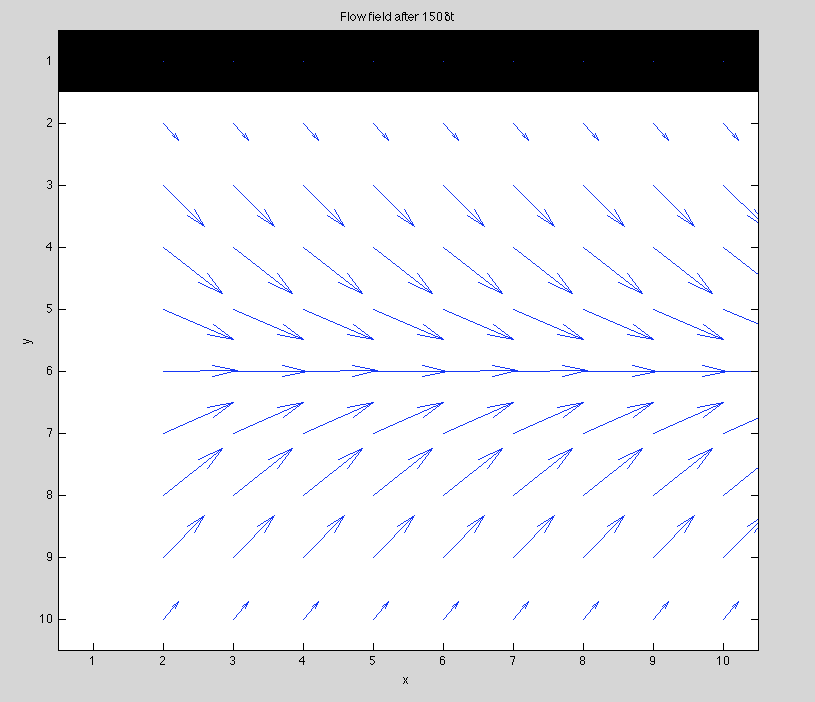
\includegraphics[width=0.30\textwidth]{./images/matlabControl.png}
\label{correctness:a}
}
\hspace{1pt}
\subfigure[NumPy]{
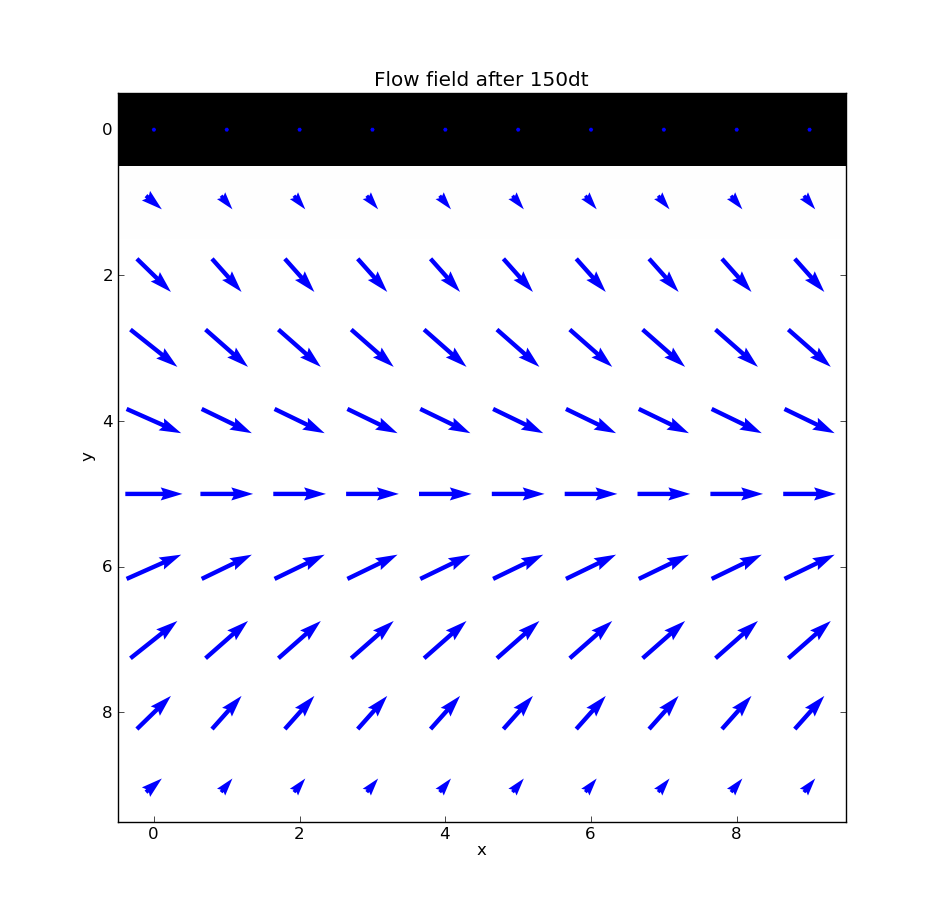
\includegraphics[width=0.27\textwidth]{./images/numpyControl.png}
\label{correctness:b}
}
\subfigure[PyCUDA]{
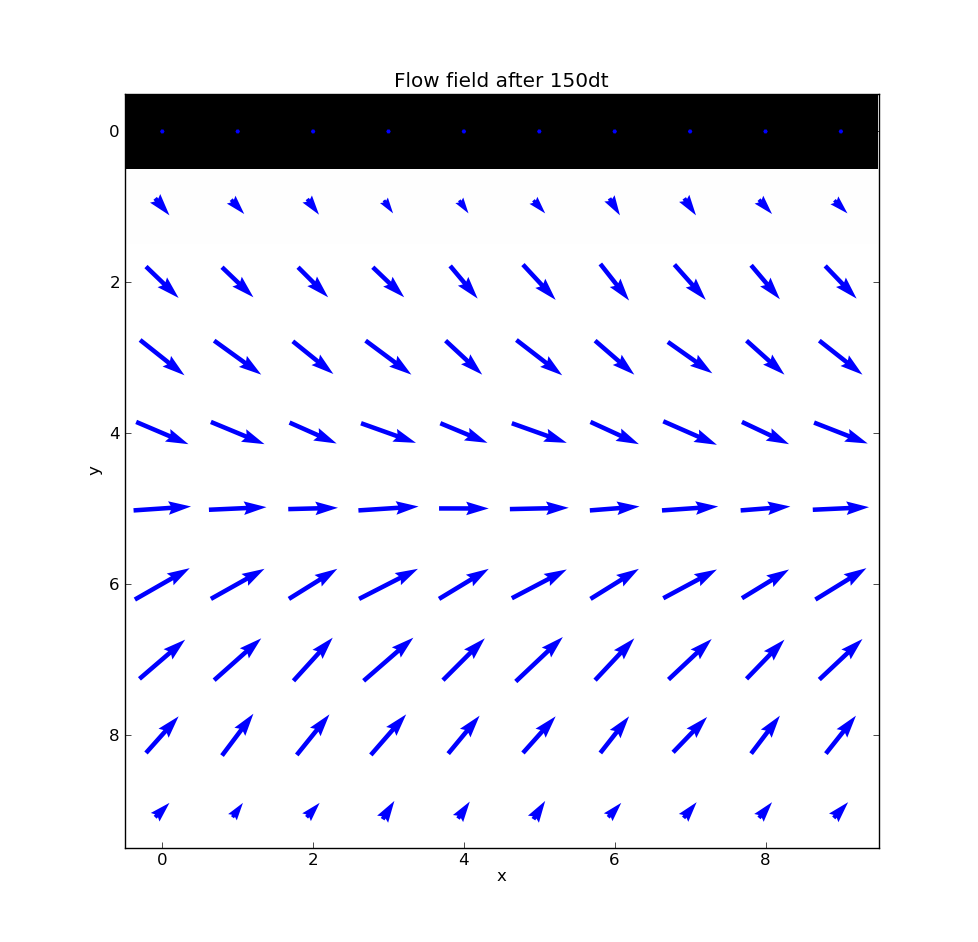
\includegraphics[width=0.27\textwidth]{./images/pycudaControl.png}
\label{correctness:c}
}
\caption{Testing that the three implementations produces the same output under equal conditions}
\label{correctness}
\end{figure}

A visual inspection of \hpref{figure}{correctness} reveals that the implementations are correct and produce the expected results according to the original Matlab implementation. There is however a small inaccuracy in the PyCUDA version on \hpref{figure}{correctness:c}, some of the velocities don't have exactly same length and direction as the NumPy version in \hpref{figure}{correctness:b}. This can be attributed to floating point inaccuracy (TODO: cite cuda best practices and maybe others).



\subsection{Optimization}
To further optimize the PyCUDA implementation one would look into different memory structures. The limiting factor in most parallel algorithms is the memory access pattern. Global memory is a relatively slow memory compared with the shared memory or the texture memory. Each of these have their specific purpose, and thought needs to be given to when to use them.

Certain parts of the data could be loaded into parts of memory more suited for the usage of that data. The \texttt{BOUND} variable is for example only read, and would benefit from a memory type which was spatial in layout. The texture memory would be a good candidate for this, and would increase the performance gain over a normal CPU-implementation.

Utilizing shared memory in each block would also provide a performance gain, but this gain would come with the cost of having to synchronize each block with adjacent blocks. Many strategies could be used to resolve this, one very common one is to calculate all changes on the border of the block first so that other blocks would not have to wait for a block to finish. (TODO: find a good quote for this in parallelism book)



\subsection{Issues/bugs}
An earlier version of the PyCUDA implementation exhibited a bug when running the kernel with a simulated field larger than the block size ($16\times16$) and not a multiple of 16 in each dimension. If the simulated field is chosen to say for example $25\times25$, the program would throw an error.

The reason for this was a mixture of miscalculations of the current thread's index, calculation of the size of the simulated field, and lacking the ability for threads to disable when there is no data for them to process. The latter is illustrated in \hpref{figure}{blockbug}. The kernels are always launched with the same block-size, and therefore will not fit with simulated fields of which the dimensions are a multiple of the block size's dimension. If the threads are not instructed not to do so, they will try to process data, regardless if there is data or not. To solve this problem a condition was inserted to check if the threads index (x and y) is within the simulated field, and therefore has data to process. 

\insfig{./images/blockbug.pdf}{0.4\textwidth}{The allocated memory is smaller than the designated block size}{blockbug}

Facing the problem of the miscalculations in the thread's index and size of the simulated field revealed that a mistake had been made. The size of the simulated field is not simply taking the amount of blocks times the dimension of a block, since this gives the total grid-size, which can be larger than the simulated field. The indexing calculations where done like so

\begin{verbatim}
int x     = threadIdx.x + blockIdx.x * blockDim.x;
int y     = threadIdx.y + blockIdx.y * blockDim.y;
int nx    = blockDim.x * gridDim.x;
int ny    = blockDim.y * gridDim.y;
int cur 	  = x + y * nx;
int size  = nx * ny;
\end{verbatim}

Both the \texttt{nx} and \texttt{ny} as well as the \texttt{size} was calculated incorrectly this way. The solution to this problem was not hard to find though. Instead of letting the threads calculate the simulated field, which anyway is impossible to infer from the grid-structure, the simulated field's dimensions were fed to the kernels as constants.

\newpage

\section{Timing}
\newpage

\section{Tests}
\newpage

\section{Code}
\newpage

\section{Running times}
\newpage

\section{Conclusion}
\newpage

\section{Appendix}

\lstset{basicstyle=\scriptsize, caption={Lattice Boltzmann Model, implemented in Matlab},label=lbmmatlab}
\lstinputlisting{./code/lbm2d.m}

\newpage
\lstset{language=Python, caption={Lattice Boltzmann Model, implemented in NumPy},label=lbmnumpy}
\lstinputlisting{./code/lbm2d.py}

\newpage
\lstset{language=Python, caption={Lattice Boltzmann Model, implemented in PyCUDA},label=lbmcuda}
\lstinputlisting{./code/lbm2dcu.py}

\bibliographystyle{plain}
\bibliography{library}
\newpage

%%%---BibTeX ---%%%
%(Compile: 1 x LaTeX 1 x Bibtex 2 x LaTex)%

\end{document}